\documentclass{standalone}
\usepackage{tikz}
\usetikzlibrary{patterns, positioning}


\begin{document}
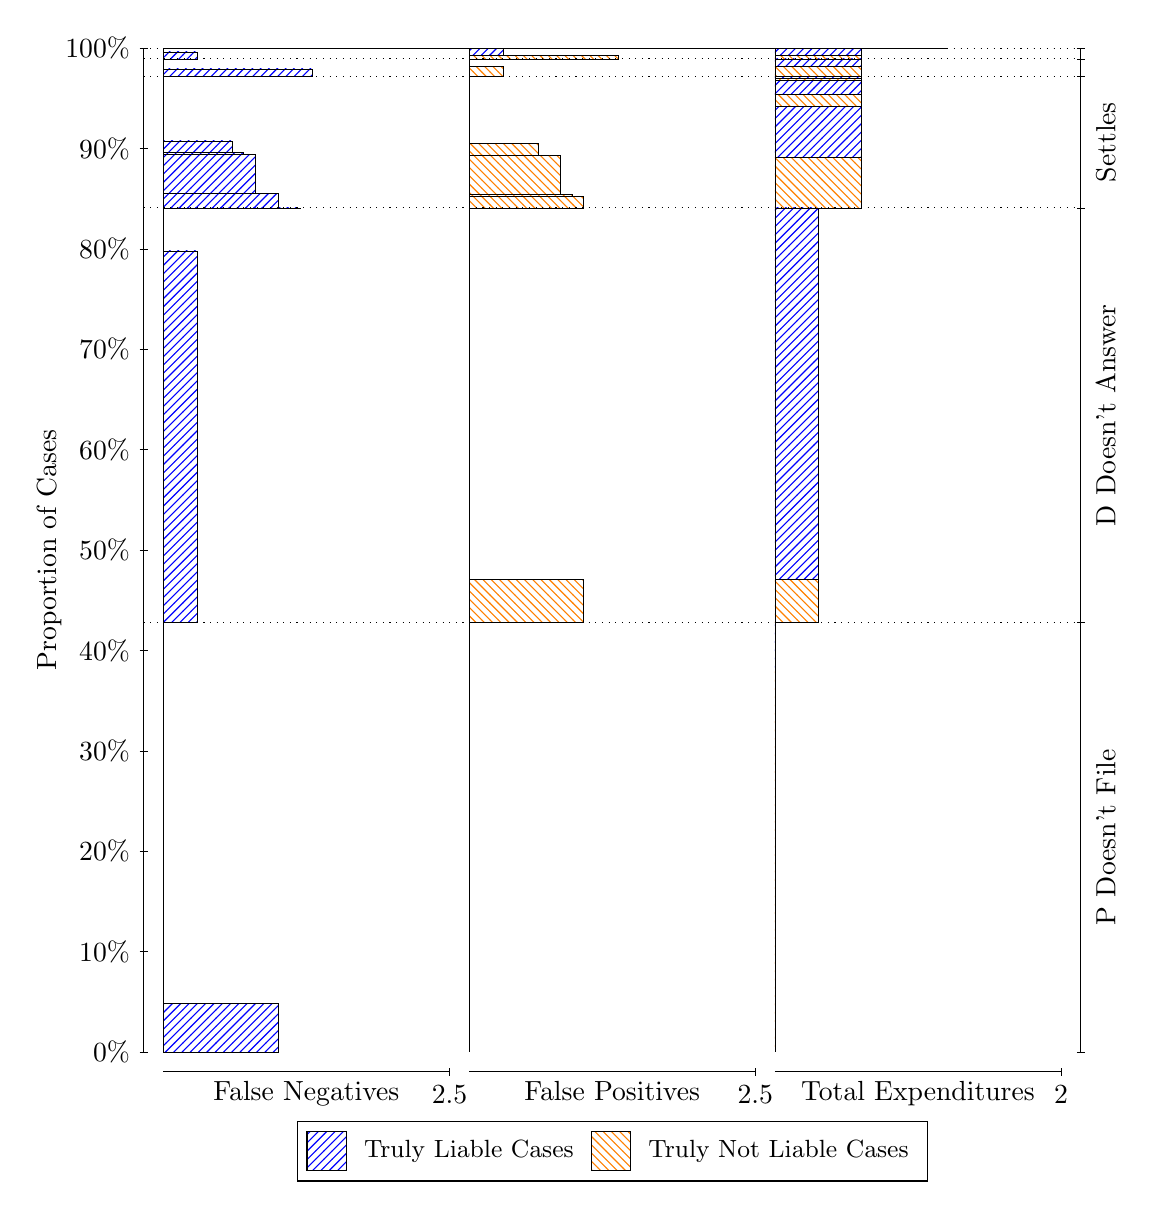
\begin{tikzpicture}
\draw[black, very thin] (1.5,1.75) -- (1.5,14.5);
\node[rotate=90, text=black, anchor=center] at (0.3, 8.125) {Proportion of Cases};
\draw[black, very thin] (1.45,1.75) -- (1.55,1.75);
\node[text=black, anchor=east] at (1.45, 1.75) {0\%};
\draw[black, very thin] (1.45,3.025) -- (1.55,3.025);
\node[text=black, anchor=east] at (1.45, 3.025) {10\%};
\draw[black, very thin] (1.45,4.3) -- (1.55,4.3);
\node[text=black, anchor=east] at (1.45, 4.3) {20\%};
\draw[black, very thin] (1.45,5.575) -- (1.55,5.575);
\node[text=black, anchor=east] at (1.45, 5.575) {30\%};
\draw[black, very thin] (1.45,6.85) -- (1.55,6.85);
\node[text=black, anchor=east] at (1.45, 6.85) {40\%};
\draw[black, very thin] (1.45,8.125) -- (1.55,8.125);
\node[text=black, anchor=east] at (1.45, 8.125) {50\%};
\draw[black, very thin] (1.45,9.4) -- (1.55,9.4);
\node[text=black, anchor=east] at (1.45, 9.4) {60\%};
\draw[black, very thin] (1.45,10.675) -- (1.55,10.675);
\node[text=black, anchor=east] at (1.45, 10.675) {70\%};
\draw[black, very thin] (1.45,11.95) -- (1.55,11.95);
\node[text=black, anchor=east] at (1.45, 11.95) {80\%};
\draw[black, very thin] (1.45,13.225) -- (1.55,13.225);
\node[text=black, anchor=east] at (1.45, 13.225) {90\%};
\draw[black, very thin] (1.45,14.5) -- (1.55,14.5);
\node[text=black, anchor=east] at (1.45, 14.5) {100\%};

\draw[black, very thin] (13.4,1.75) -- (13.4,14.5);
\draw[black, very thin] (13.35,1.75) -- (13.45,1.75);
\node[anchor=west] at (13.35, 1.75) {};
\draw[black, very thin] (13.35,7.2052) -- (13.45,7.2052);
\node[anchor=west] at (13.35, 7.2052) {};
\draw[black, very thin] (13.35,12.47) -- (13.45,12.47);
\node[anchor=west] at (13.35, 12.47) {};
\draw[black, very thin] (13.35,14.141) -- (13.45,14.141);
\node[anchor=west] at (13.35, 14.141) {};
\draw[black, very thin] (13.35,14.363) -- (13.45,14.363);
\node[anchor=west] at (13.35, 14.363) {};
\draw[black, very thin] (13.35,14.496) -- (13.45,14.496);
\node[anchor=west] at (13.35, 14.496) {};
\draw[black, very thin] (13.35,14.497) -- (13.45,14.497);
\node[anchor=west] at (13.35, 14.497) {};
\draw[black, very thin] (13.35,14.5) -- (13.45,14.5);
\node[anchor=west] at (13.35, 14.5) {};

\draw[black, very thin, pattern color=blue, pattern=north east lines] (1.75,1.75) rectangle (3.2033,2.368);
\draw[black, very thin, pattern color=orange, pattern=north west lines] (1.75,2.368) rectangle (1.75,7.2052);
\draw[black, very thin, pattern color=blue, pattern=north east lines] (1.75,7.2052) rectangle (2.186,11.924);
\draw[black, very thin, pattern color=orange, pattern=north west lines] (1.75,11.924) rectangle (1.75,12.47);
\draw[black, very thin, pattern color=blue, pattern=north east lines] (1.75,12.47) rectangle (3.494,12.471);
\draw[black, very thin, pattern color=blue, pattern=north east lines] (1.75,12.471) rectangle (3.3487,12.471);
\draw[black, very thin, pattern color=blue, pattern=north east lines] (1.75,12.471) rectangle (3.2033,12.65);
\draw[black, very thin, pattern color=blue, pattern=north east lines] (1.75,12.65) rectangle (3.058,12.651);
\draw[black, very thin, pattern color=blue, pattern=north east lines] (1.75,12.651) rectangle (2.9127,13.147);
\draw[black, very thin, pattern color=blue, pattern=north east lines] (1.75,13.147) rectangle (2.7673,13.172);
\draw[black, very thin, pattern color=blue, pattern=north east lines] (1.75,13.172) rectangle (2.622,13.32);
\draw[black, very thin, pattern color=orange, pattern=north west lines] (1.75,13.32) rectangle (1.75,14.141);
\draw[black, very thin, pattern color=blue, pattern=north east lines] (1.75,14.141) rectangle (3.6393,14.236);
\draw[black, very thin, pattern color=orange, pattern=north west lines] (1.75,14.236) rectangle (1.75,14.363);
\draw[black, very thin, pattern color=blue, pattern=north east lines] (1.75,14.363) rectangle (2.186,14.452);
\draw[black, very thin, pattern color=orange, pattern=north west lines] (1.75,14.452) rectangle (1.75,14.496);
\draw[black, very thin, pattern color=blue, pattern=north east lines] (1.75,14.496) rectangle (5.8193,14.497);
\draw[black, very thin, pattern color=orange, pattern=north west lines] (1.75,14.497) rectangle (1.75,14.497);
\draw[black, very thin, pattern color=orange, pattern=north west lines] (1.75,14.497) rectangle (1.75,14.498);
\draw[black, very thin, pattern color=blue, pattern=north east lines] (1.75,14.498) rectangle (1.75,14.5);
\draw[black, very thin, pattern color=orange, pattern=north west lines] (5.6333,1.75) rectangle (5.6333,6.5872);
\draw[black, very thin, pattern color=blue, pattern=north east lines] (5.6333,6.5872) rectangle (5.6333,7.2052);
\draw[black, very thin, pattern color=orange, pattern=north west lines] (5.6333,7.2052) rectangle (7.0867,7.7511);
\draw[black, very thin, pattern color=blue, pattern=north east lines] (5.6333,7.7511) rectangle (5.6333,12.47);
\draw[black, very thin, pattern color=orange, pattern=north west lines] (5.6333,12.47) rectangle (7.0867,12.618);
\draw[black, very thin, pattern color=orange, pattern=north west lines] (5.6333,12.618) rectangle (6.9413,12.641);
\draw[black, very thin, pattern color=orange, pattern=north west lines] (5.6333,12.641) rectangle (6.796,13.136);
\draw[black, very thin, pattern color=orange, pattern=north west lines] (5.6333,13.136) rectangle (6.6507,13.136);
\draw[black, very thin, pattern color=orange, pattern=north west lines] (5.6333,13.136) rectangle (6.5053,13.29);
\draw[black, very thin, pattern color=orange, pattern=north west lines] (5.6333,13.29) rectangle (6.36,13.29);
\draw[black, very thin, pattern color=orange, pattern=north west lines] (5.6333,13.29) rectangle (6.2147,13.291);
\draw[black, very thin, pattern color=blue, pattern=north east lines] (5.6333,13.291) rectangle (5.6333,14.141);
\draw[black, very thin, pattern color=orange, pattern=north west lines] (5.6333,14.141) rectangle (6.0693,14.267);
\draw[black, very thin, pattern color=blue, pattern=north east lines] (5.6333,14.267) rectangle (5.6333,14.363);
\draw[black, very thin, pattern color=orange, pattern=north west lines] (5.6333,14.363) rectangle (7.5227,14.406);
\draw[black, very thin, pattern color=blue, pattern=north east lines] (5.6333,14.406) rectangle (6.0693,14.496);
\draw[black, very thin, pattern color=orange, pattern=north west lines] (5.6333,14.496) rectangle (5.6333,14.497);
\draw[black, very thin, pattern color=blue, pattern=north east lines] (5.6333,14.497) rectangle (5.6333,14.497);
\draw[black, very thin, pattern color=orange, pattern=north west lines] (5.6333,14.497) rectangle (9.7027,14.498);
\draw[black, very thin, pattern color=blue, pattern=north east lines] (5.6333,14.498) rectangle (8.2493,14.5);
\draw[black, very thin, pattern color=orange, pattern=north west lines] (9.5167,1.75) rectangle (9.5167,6.5872);
\draw[black, very thin, pattern color=blue, pattern=north east lines] (9.5167,6.5872) rectangle (9.5167,7.2052);
\draw[black, very thin, pattern color=orange, pattern=north west lines] (9.5167,7.2052) rectangle (10.062,7.7511);
\draw[black, very thin, pattern color=blue, pattern=north east lines] (9.5167,7.7511) rectangle (10.062,12.47);
\draw[black, very thin, pattern color=orange, pattern=north west lines] (9.5167,12.47) rectangle (10.607,13.113);
\draw[black, very thin, pattern color=blue, pattern=north east lines] (9.5167,13.113) rectangle (10.607,13.757);
\draw[black, very thin, pattern color=orange, pattern=north west lines] (9.5167,13.757) rectangle (10.607,13.912);
\draw[black, very thin, pattern color=blue, pattern=north east lines] (9.5167,13.912) rectangle (10.607,14.093);
\draw[black, very thin, pattern color=orange, pattern=north west lines] (9.5167,14.093) rectangle (10.607,14.116);
\draw[black, very thin, pattern color=blue, pattern=north east lines] (9.5167,14.116) rectangle (10.607,14.141);
\draw[black, very thin, pattern color=orange, pattern=north west lines] (9.5167,14.141) rectangle (10.607,14.267);
\draw[black, very thin, pattern color=blue, pattern=north east lines] (9.5167,14.267) rectangle (10.607,14.363);
\draw[black, very thin, pattern color=orange, pattern=north west lines] (9.5167,14.363) rectangle (10.607,14.406);
\draw[black, very thin, pattern color=blue, pattern=north east lines] (9.5167,14.406) rectangle (10.607,14.496);
\draw[black, very thin, pattern color=orange, pattern=north west lines] (9.5167,14.496) rectangle (11.697,14.497);
\draw[black, very thin, pattern color=blue, pattern=north east lines] (9.5167,14.497) rectangle (11.697,14.497);
\draw[black, very thin, pattern color=orange, pattern=north west lines] (9.5167,14.497) rectangle (11.697,14.498);
\draw[black, very thin, pattern color=blue, pattern=north east lines] (9.5167,14.498) rectangle (11.697,14.5);
\draw[black, dotted] (1.5,7.2052) -- (13.4,7.2052);
\draw[black, dotted] (1.5,12.47) -- (13.4,12.47);
\draw[black, dotted] (1.5,14.141) -- (13.4,14.141);
\draw[black, dotted] (1.5,14.363) -- (13.4,14.363);
\draw[black, dotted] (1.5,14.496) -- (13.4,14.496);
\draw[black, dotted] (1.5,14.497) -- (13.4,14.497);
\draw[black, very thin] (1.75,1.5) -- (5.3833,1.5);
\node[text=black, anchor=north] at (3.5667, 1.5) {False Negatives};
\draw[black, very thin] (5.3833,1.45) -- (5.3833,1.55);
\node[text=black, anchor=north] at (5.3833, 1.45) {2.5};

\draw[black, very thin] (5.6333,1.5) -- (9.2667,1.5);
\node[text=black, anchor=north] at (7.45, 1.5) {False Positives};
\draw[black, very thin] (9.2667,1.45) -- (9.2667,1.55);
\node[text=black, anchor=north] at (9.2667, 1.45) {2.5};

\draw[black, very thin] (9.5167,1.5) -- (13.15,1.5);
\node[text=black, anchor=north] at (11.333, 1.5) {Total Expenditures};
\draw[black, very thin] (13.15,1.45) -- (13.15,1.55);
\node[text=black, anchor=north] at (13.15, 1.45) {2};

\node[text=black, centered, rotate=90] at (13.72, 4.4776) {P Doesn't File};
\node[text=black, centered, rotate=90] at (13.72, 9.8377) {D Doesn't Answer};
\node[text=black, centered, rotate=90] at (13.72, 13.305) {Settles};





\draw (7.449999999999999,1.5) node[draw=none] (baseCoordinate) {};
\begin{scope}[align=center]
        \matrix[scale=0.5, draw=black, below=0.5cm of baseCoordinate, nodes={draw}, column sep=0.1cm]{
            \node[rectangle, draw, minimum width=0.5cm, minimum height=0.5cm, pattern color=blue, pattern=north east lines] {}; &
            \node[draw=none, font=\small, text=black] (B) {Truly Liable Cases}; &
            \node[rectangle, draw, minimum width=0.5cm, minimum height=0.5cm, pattern color=orange, pattern=north west lines] {}; &
            \node[draw=none, font=\small, text=black] (B) {Truly Not Liable Cases}; \\
            };
\end{scope}

\end{tikzpicture}
\end{document}